%\documentclass[10pt,handout]{beamer}
\documentclass[10pt]{beamer}
\usepackage{babel} % Anpassa efter svenska. Ger svensk logga.
\usepackage[utf8]{inputenc} % Anpassa efter linux
\usepackage{graphicx}
\usepackage{../common/beamerthemeUppsala}
%\usecolortheme{UU} % Anpassa efter UU:s frger och logga
%\hypersetup{pdfpagemode=FullScreen} % Adobe Reader ska ppna fullskrm
\setbeamertemplate{itemize items}[circle]

% \usepackage{beamerthemesplit}
\usepackage{amsmath}
\usepackage{amssymb}
% \usepackage{graphics}
% \usepackage{graphicx}
% \usepackage{epsfig}
% \usepackage[latin1]{inputenc}
 \usepackage{color}
% \usepackage{fancybox}
% \usepackage{psfrag}
% \usepackage[english]{babel}
 \setbeamertemplate{footline}{\hfill\insertframenumber/\inserttotalframenumber}


% Read in commands
% Course settings
\newcommand{\currentsemester}{Autumn 2024}

% New commands
\newcommand{\bfm}[1]   {\mbox{\boldmath{${#1}$}}}
\newcommand{\Prob}   {\mbox{\textnormal{P}}}
\newcommand{\uured}[1]{\textcolor{uured}{#1}}

% Eqds
\def\eqd{\,{\buildrel d \over =}\,}

% Math operators
\DeclareMathOperator{\E}{\mathbb{E}}
\DeclareMathOperator{\V}{\mathbb{V}}



%%%%%%%%%%%%%%%%%%%%%%%%%%%%%%%%%%%%%%%%%%%%%%%%%%%%%%%%%%%%%%%%%%

\setlength{\parskip}{3mm}
\title[]{{\color{black}Machine learning -- Large Language Models}}
\author[]{M{\aa}ns Magnusson\\Department of Statistics, Uppsala University}
\date{\currentsemester}


\begin{document}

\frame{\titlepage
% \thispagestyle{empty}
}

%%%%%%%%%%%%%%%%%%%%%%%%%%%%%%%%%%%%%%%%%%%%%%%%%%%%%%%%%%%%%%%%%%




\section{Introduction} % to Large Language Models

\begin{frame}{What is a Large Language Model?}

\begin{itemize}
  \item Large Language Models (LLM) are commonly defined as:
  \begin{itemize}
      \item large natural language models (usually transformer-based)
      \pause
      \item generative and autoregressive, predicting a token at a time, based on previous \uured{context}
      \pause
      \item having some ability to achieve \uured{general-purpose language "understanding"}
      \item show \uured{emergent} abilities to solve other more complex tasks
      \pause
      \item fit for few-shot learning and \uured{incontext} learning
      \pause
      \item pre-trained on very large data
  \end{itemize}
  \item Compared to pretrained language models (PLM), LLMs are
  \begin{itemize}
      \item larger (billions or trillions, rather than millions of parameters), in practice only possible to train by a few persons
      \item possible to use for in-context learning
      \item usually interacted with through the prompt
  \end{itemize}
\end{itemize}

\end{frame}

\begin{frame}{Historical development}

\begin{figure}[h]
\centering
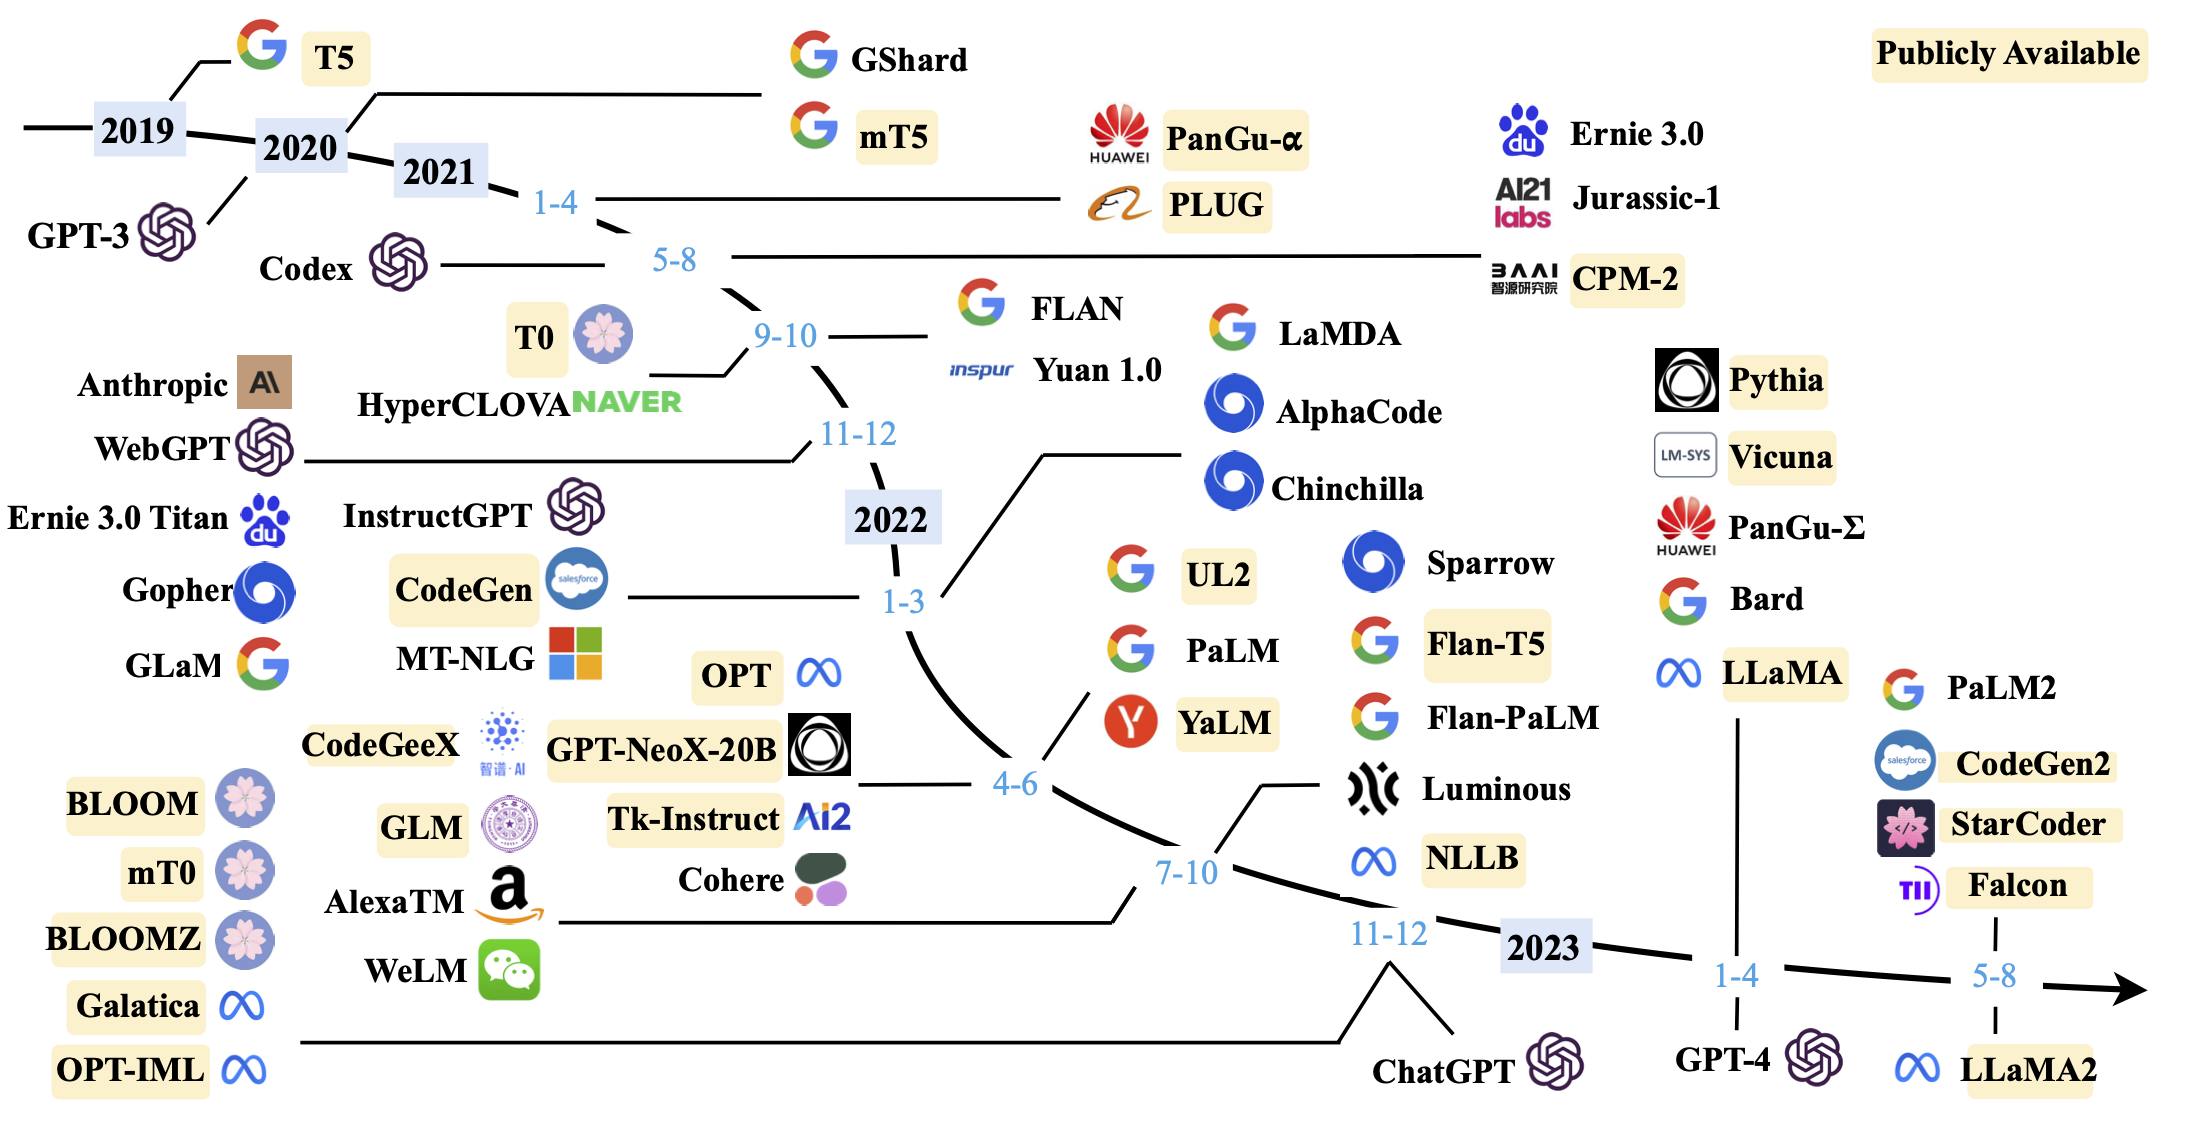
\includegraphics[width=0.99\textwidth]{fig/fig2_zhao_2023}
\caption{The development of LLMs (Figure 2, Zhao et al., 2023)}
\end{figure}

\begin{itemize}
    \item Milestones (subjective): GPT-3, GPT-4, chatGPT, Llama 2
\end{itemize}

\end{frame}

\begin{frame}{A subset of current LLMs}

\begin{figure}[h]
\centering
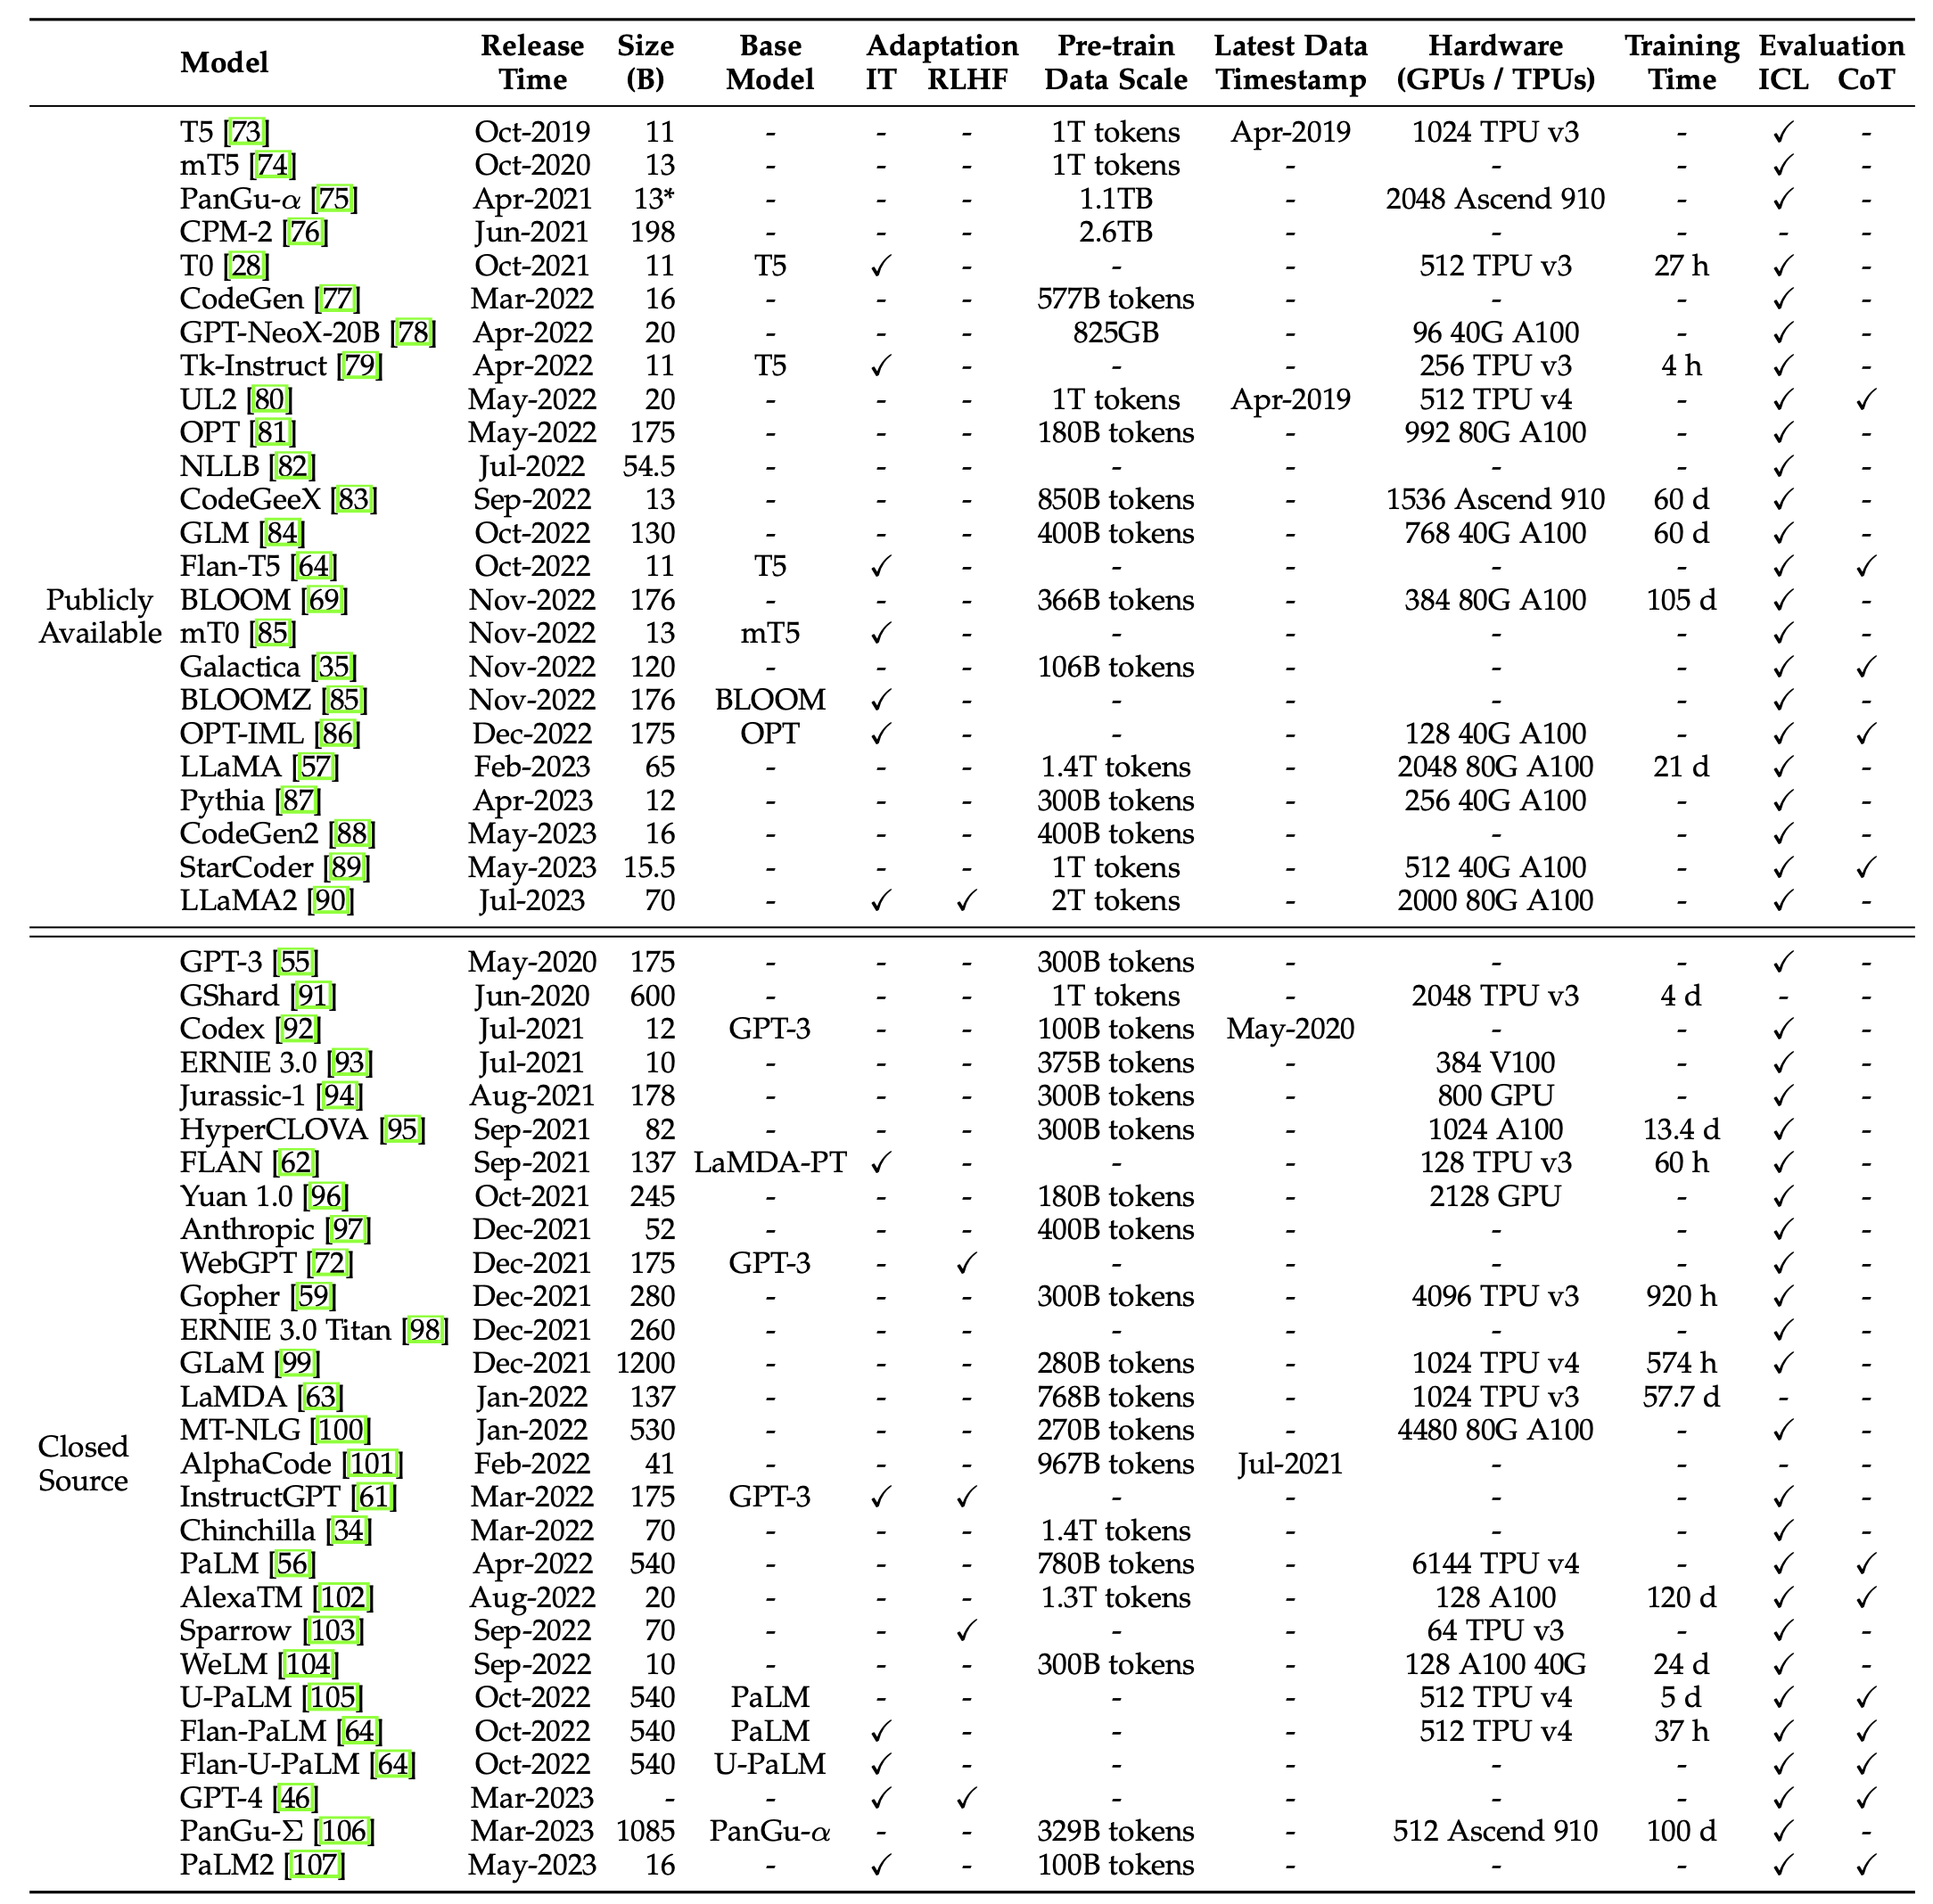
\includegraphics[width=0.82\textwidth]{fig/tab1_zhao_2023}
\caption{Statistics of LLMs (Table 1, Zhao et al., 2023)}
\end{figure}

\end{frame}

\begin{frame}{Examples of LLM prompting}

Examples:
\begin{enumerate}
\item Can you please add 113329 and 719292? (true is 832621)
\item Who is Olof Palme? Please respond both in English and Swedish.
\end{enumerate}

\centering

\vspace{5mm}

\href{https://www.llama2.ai/}{Llama 2}

\vspace{10mm}

\href{https://chat.openai.com/}{chatGPT}

\end{frame}


\begin{frame}{Why is this working now?}

\begin{itemize}
\item Scaling of pretrained models, performals (loss) improves by:
\begin{itemize}
\item Larger models (GPT3 175B, PaLM 540B)
\item Larger datasets
\item More computation
\item Scaling laws (CITE, CITE) show that all three are important\\
\uured{Can we connect this back to the standard ML framework?}
% Scaling laws has shown that all three matters and is of importance.
\end{itemize}
\pause
\item Fine-tuning for tuning models to follow instructions (InstructGPT)
\end{itemize}

\end{frame}


%\begin{frame}{Scaling laws}

%Extensive research has shown that scaling can largely improve the model capacity of LLMs

% Scale Matters/ Scaling laws p 4 in Zhao
% model performance with respective to three major factors
% namely model size (N), dataset size (D),

%\end{frame}


\begin{frame}{Emergant abilities}
% Emergent abilities
% p 4 in Zhao
\begin{itemize}
\item "the abilities that are not present in small models but arise in large models" (Zhao et al, 2023)
\item One of the main differences between LLMs and PLMs
\item Examples:
\begin{itemize}
\item In-context learning (basis for prompting)
\item Instruction following % "LaMDA-PT started to significantly outperform the untuned one on unseen tasks when the model size reached 68B, but not for 8B or smaller model sizes."
\item Step-by-step reasoning
\end{itemize}
\end{itemize}



\end{frame}


\begin{frame}{In-context learning (ICL)}

\begin{itemize}
\item Learning tasks in the actual context (think chat).
\item We demonstrate what to do with a few examples
\item The model learn what todo \uured{in context}
\item ICL only prompts LLMs for utilization
\item Let
\[
D_k = \left(f(x_1, y_1),...,f(x_k, y_k) \right)
\]
then
\[
\hat{y} = \text{LLM}(I, \underbrace{\left(f(x_1, y_1),...,f(x_k, y_k)\right)}_{demonstrations}, \underbrace{f(x_{k+1}}_{input} , ...)
\]
where $I$ is the general instructions.
\item The problem is to design the instructions in a good way.
\item What happens under the hood? We position the model in embeddings space.
\item Crazy examples: "Take a deep breath and think hard."
\item Several studies have shown that the effectiveness of ICL is highly affected by the design of demonstrations %[350, 370, 371]

\end{itemize}

% TODO: A comprehensive review of ICL has been presented in the survey paper [50], and we suggest the readers refer- ring to it for a more general, detailed discussion on this topic.
% In-context learning
% 6.1 Zhao

\end{frame}


\begin{frame}{Demonstration}
% Zhao see 6.1.2.
% the selected demon- stration examples in ICL should contain sufficient informa- tion about the task to solve as well as be relevant to the test query, for the above two selection approaches.

\begin{itemize}
\item  Demonstration selection
\begin{itemize}
\item Not well explored: k-NN based retriever to select examples
\item To resolve this issue, diversity-based selection strategies are proposed to choose the most representative set of examples for specific tasks
\item LLM-based methods to choose examples. E.g. ome recent studies employ LLM itself as the demonstration generator without human intervention
\end{itemize}
\item Demonstration format
\begin{itemize}
\item "Lets think step by step", "Take a deep breath and think."
\end{itemize}
\item Demonstration order
\begin{itemize}
\item Indications of recency bias (they are prone to repeat answers that are near the end of demonstrations)
\item Why?
\end{itemize}

\end{itemize}


\end{frame}




\begin{frame}{Chain of thought (CoT) prompting}

% Zhao Section 6.2

\begin{itemize}
\item Prompting strategy to improve performance in "reasoning"
\item Incorporates intermediate reasoning steps that can lead to the final output
\item instead of (input, output), we use (input, cot, output)
\item Zero-shot CoT: "Lets think step by step"
\end{itemize}

\begin{figure}[h]
\centering
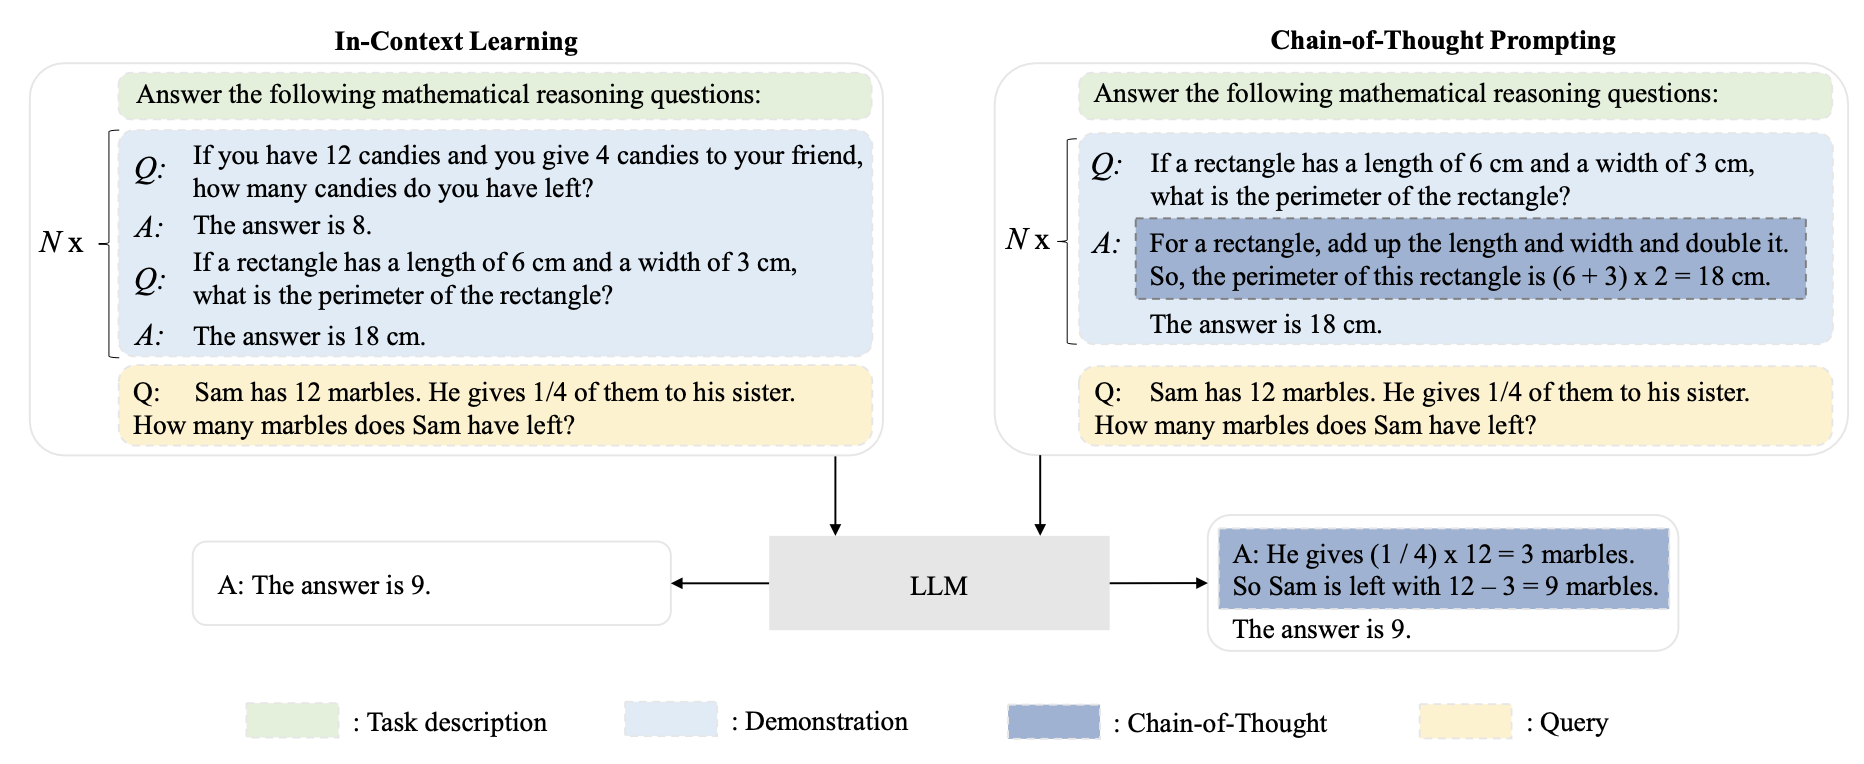
\includegraphics[width=0.99\textwidth]{fig/zhao_2023_fig12}
\caption{ICL vs CoT (Figure 12, Zhao et al., 2023)}
\end{figure}

\end{frame}



\subsection{Hallucinations}

\begin{frame}{Hallucinations: What is it?}
% What is it?
\begin{itemize}
\item "Generated text that is fluent and natural but unfaithful"
\item LLMs are prone to generate untruthful information, often called \uured{hallicinations} that
\begin{itemize}
\item logically contradicts the source content (intrinsic hallucination)
\item cannot be verified by the available source (intrinsic hallucination)
\end{itemize}
\item If LLMs are used for factual information - this is a major problem.
\item See Huang et al (2023) for a survey on hallucination %https://arxiv.org/pdf/2311.05232.pdf
\end{itemize}

\begin{figure}[h]
\centering
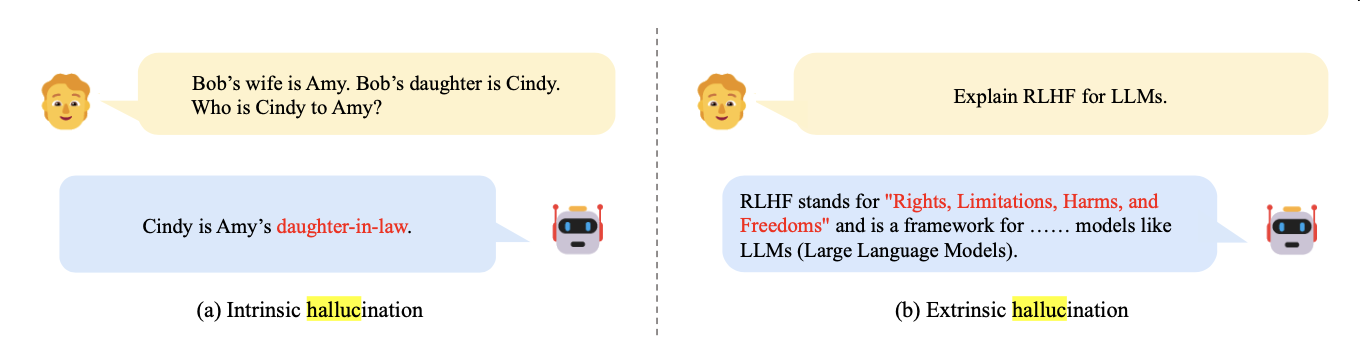
\includegraphics[width=0.99\textwidth]{fig/zhou_2023_fig14}
\caption{RLHF (Zhao, 2023, Figure 14)}
\end{figure}

\end{frame}


% intrinsic and extrinsic hallucinations [241]
% . In the former, the generated text logically contradicts the source content. In the latter, we cannot verify the output correctness from the provided source; the source content does not provide enough information to assess the out- put, which is, therefore, under-determined.

%In generating factual texts, a challenging issue is hallucination generations [518], where the generated information is either in conflict with the existing source (intrinsic hallucination) or cannot be verified by the avail- able source (extrinsic hallucination),

% LLMs are prone to generate untruthful informa- tion that either conflicts with the existing source or cannot be verified by the available source. Even the most powerful LLMs such as ChatGPT face great challenges in migrating the halluci- nations the generated texts. This issue can be partially alleviated by special approaches such as alignment tuning and tool utilization.

% Zhao
% Hallucinations
% Kaddour (2023): 2.8, Fig 7


\begin{frame}{Hallucinations: Example}


\begin{figure}[h]
\centering
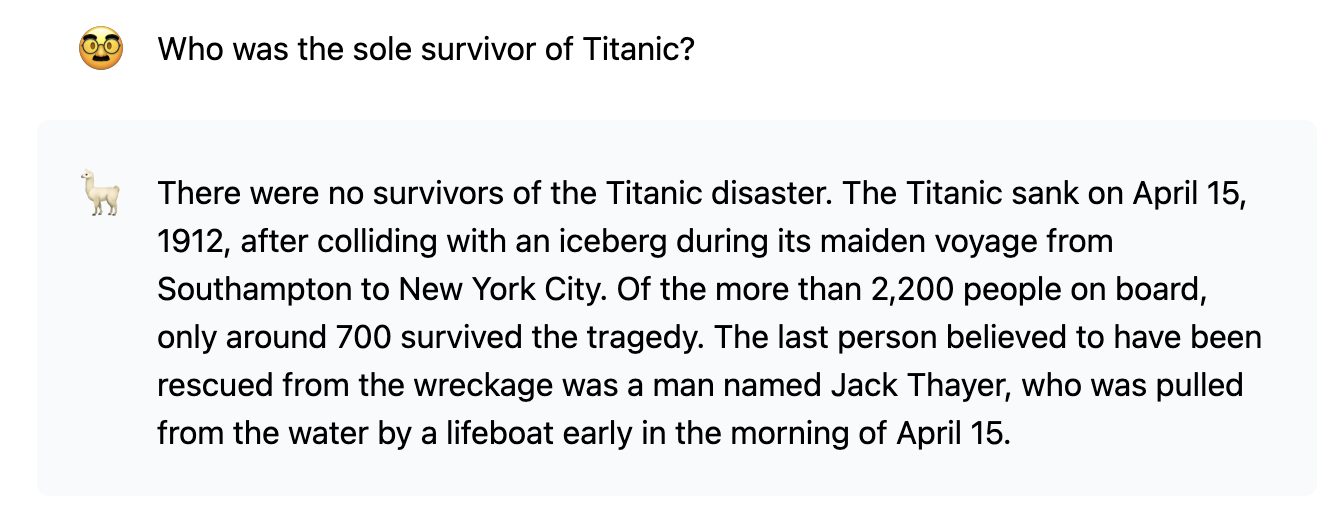
\includegraphics[width=0.99\textwidth]{fig/hall_llama7B}
\caption{Hallucinations with Llama 2 (7B, from 2023-11-25)}
\end{figure}

\end{frame}

\begin{frame}{Hallucinations: Example}


\begin{figure}[h]
\centering
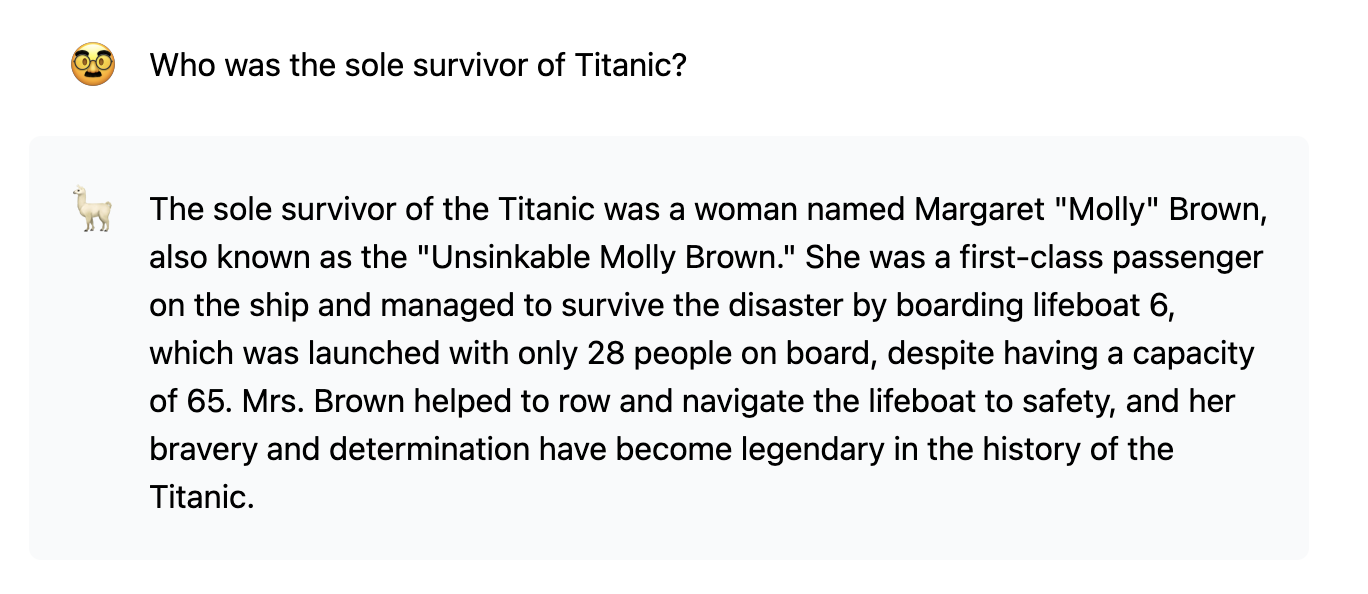
\includegraphics[width=0.99\textwidth]{fig/hall_llama70B}
\caption{Hallucinations with Llama 2 (70B, from 2023-11-25)}
\end{figure}

\end{frame}

\begin{frame}{Hallucinations: Example}

\begin{figure}[h]
\centering
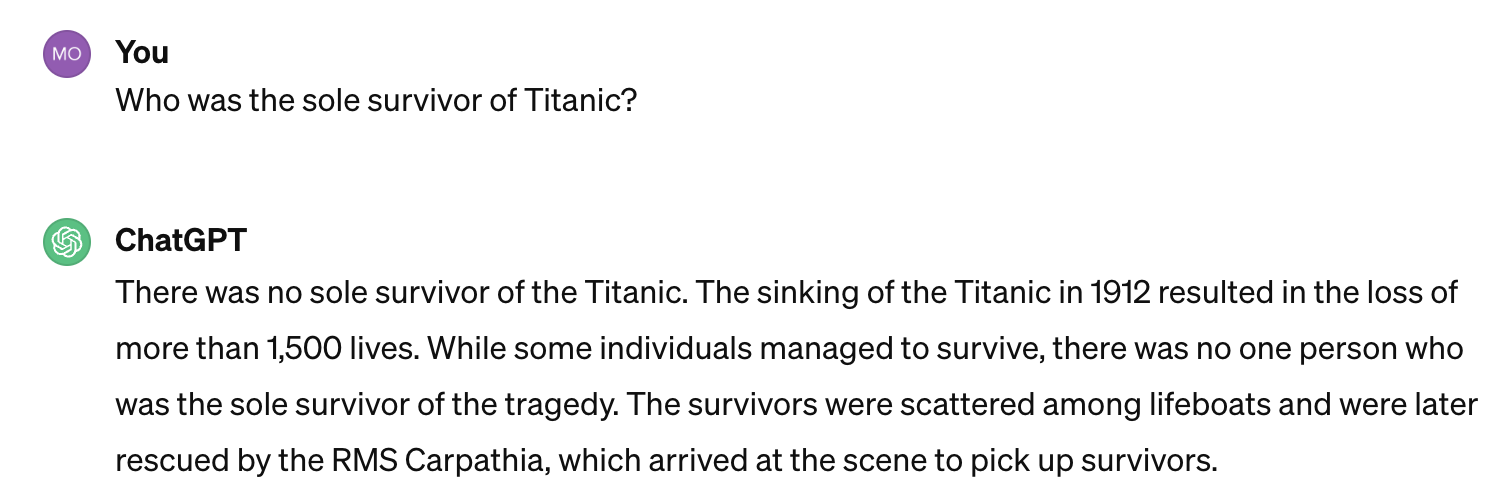
\includegraphics[width=0.99\textwidth]{fig/hall_gpt35}
\caption{Hallucinations with GPT3.5 (from 2023-11-25)}
\end{figure}

\end{frame}

\begin{frame}{Hallucinations: Causes and Mitigations}
% What is it?
\begin{itemize}
\item LLMs are not trained for factual correctness
\item Knowledge changes over time - pretraining takes a lot of time. %The parametric knowledge of LLMs is hard to be updated in a timely manner. Augmenting LLMs with external knowledge sources is a practical approach to tackling the issue. However, how to effectively update knowledge within LLMs remains an open research problem.
\end{itemize}
\begin{figure}[h]
\centering
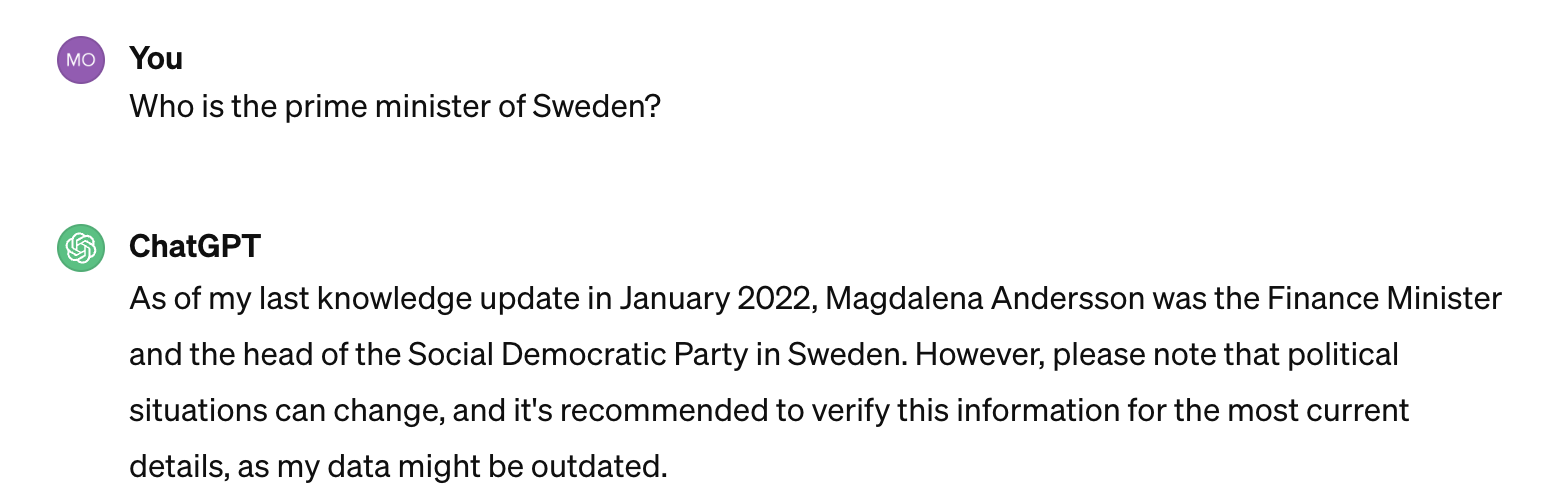
\includegraphics[width=0.99\textwidth]{fig/hall2_gpt35}
\caption{Hallucinations with GPT3.5 (from 2023-11-26)}
\end{figure}
\begin{itemize}
\pause
\item Decoding strategies % Dziri et al. [136] observe a positive correlation between increased diversity in response generation and hallucinations.
\item Retrieval-augmented generation (RAG) % For (i), a retriever module retrieves the top-k relevant documents (or passages) for a query from a large corpus of text. Then, for (ii), we feed these retrieved documents to the language model together with the initial prompt. In theory, using an external data source may also make it eas- ier to interpret which knowledge is retrieved and update it without tediously fine-tuning the model.
\end{itemize}

\end{frame}


\section{Architectures}

\begin{frame}{The transformer (Vaswani et al., 2017)}

\begin{figure}[h]
\centering
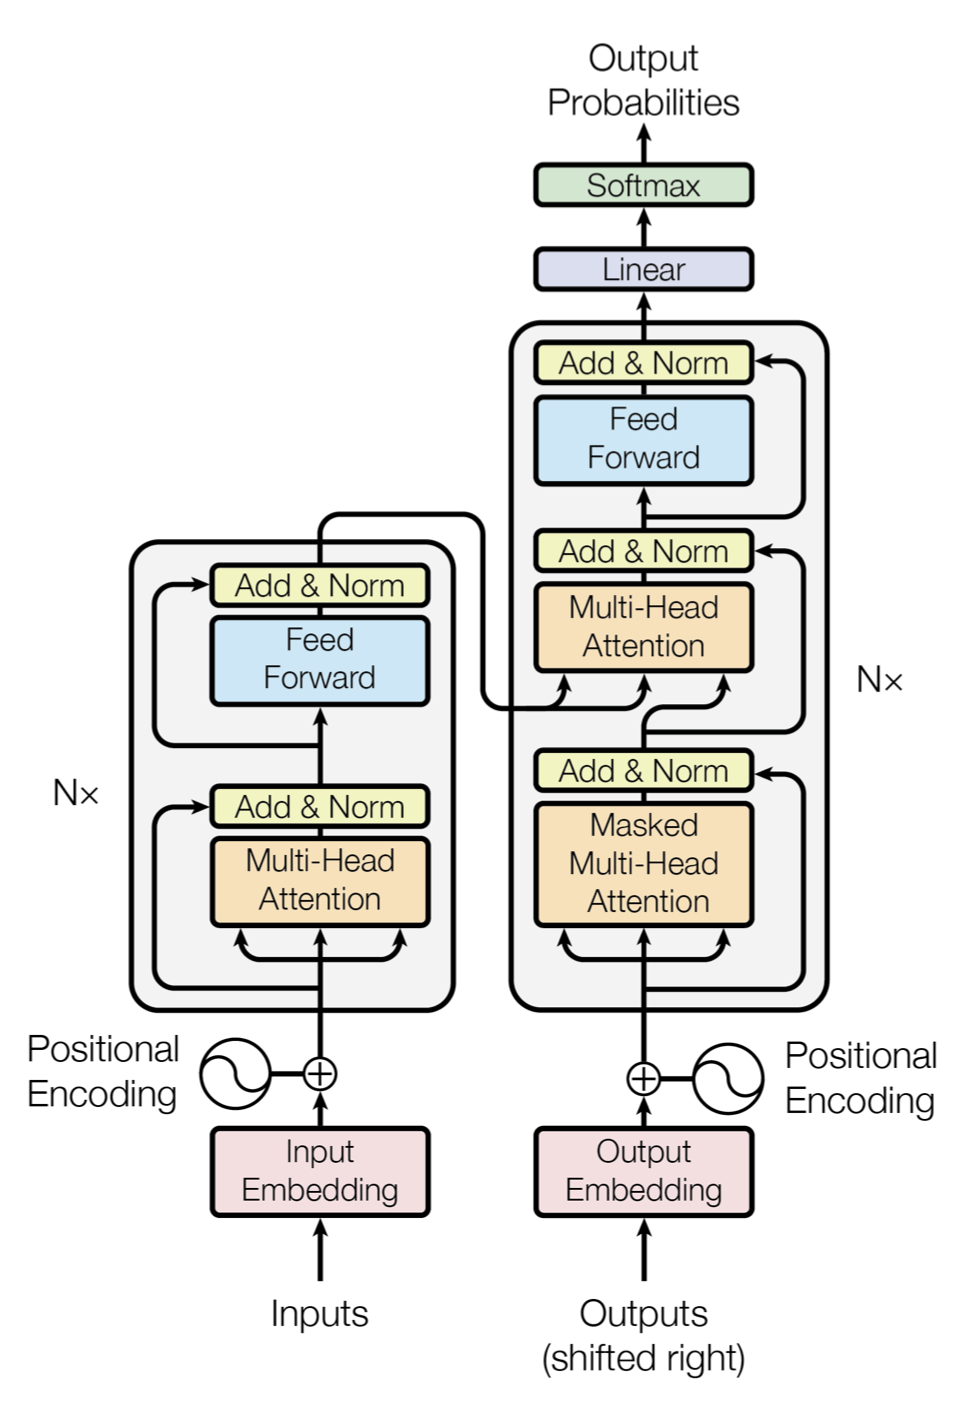
\includegraphics[width=0.6\textwidth]{fig/Vaswani_1_transformer}
\caption{The transformer (Vaswani et al., 2017)}
\end{figure}

\end{frame}

\begin{frame}{Architectures}
% TODO: Add images from the Illustrated GPT-2

\begin{itemize}
\item LLMs are usually based on the transformer \uured{decoder}
\item "Decoder-only architectures"
\item Why autoregressive decoders? Predicting the next word.
\end{itemize}

\end{frame}


\begin{frame}{Architecture configurations}

\begin{figure}[h]
\centering
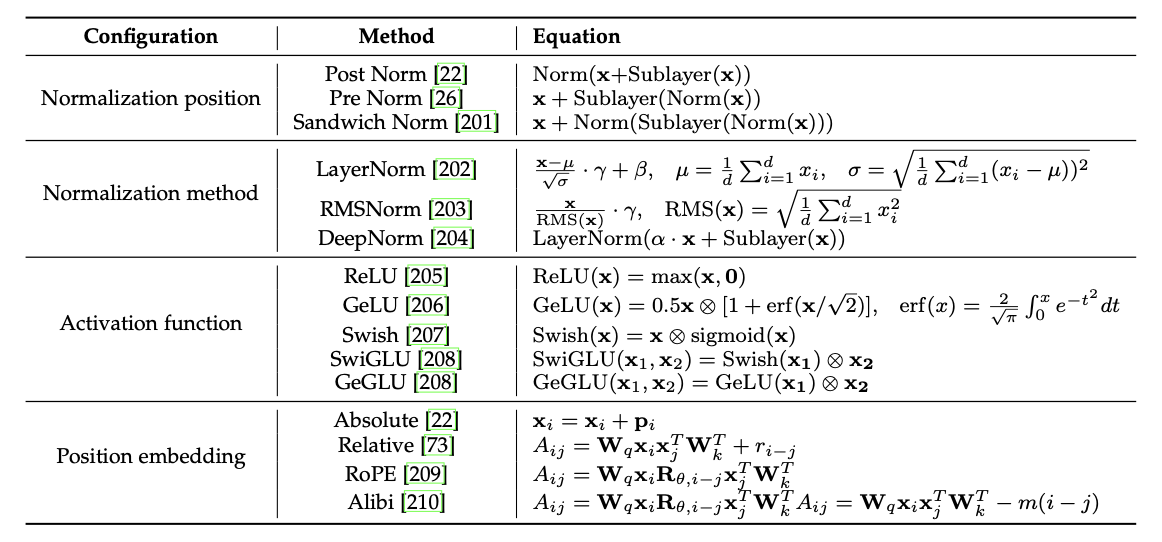
\includegraphics[width=0.99\textwidth]{fig/zhou_2023_tab4}
\caption{Common configurations (Zhou et al., 2023)}
\end{figure}
where "sublayer" indicates the previous layer in the network.
%\begin{itemize}
%\item
%\end{itemize}

\end{frame}


\begin{frame}{Common models and their configuration}

\begin{figure}[h]
\centering
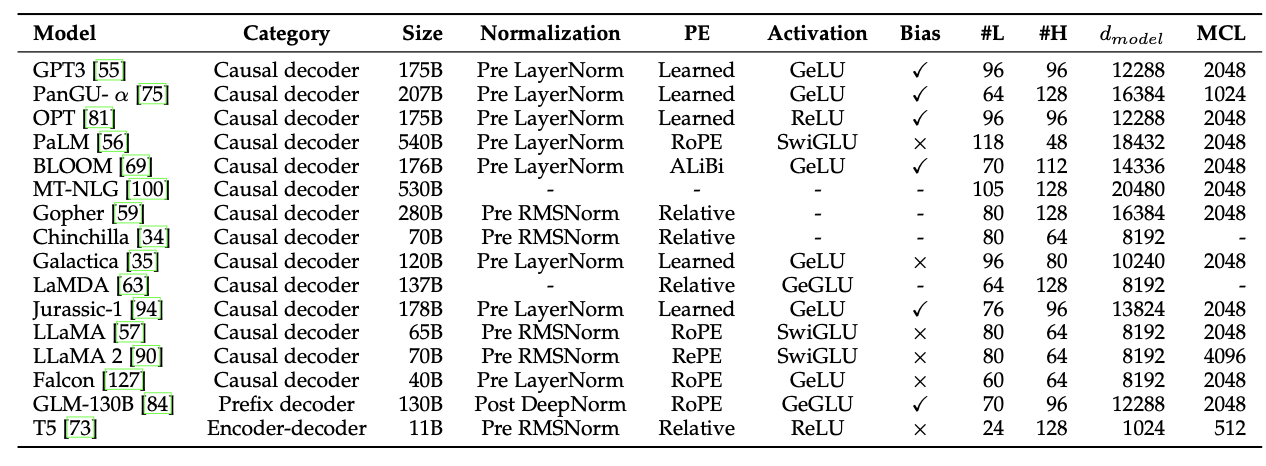
\includegraphics[width=0.99\textwidth]{fig/zhou_2023_tab3}
\caption{Common configurations (Zhou et al., 2023, Table 3)}
\end{figure}

\end{frame}


\begin{frame}{Decoding (word generation)}

\begin{itemize}
\item LLMs are trained to predict the next word (called decoding), i.e the discret probability model (pmf)
\[
p_{x,i} = P(x_i|\mathbf{x}_{j<i})
\]
\item Two approaches to generate/decode:
\begin{description}
\item[greedy] $x_i = \arg_x \max P(x|\mathbf{x}_{j<i})$
\item[sampling] $x_i \sim P(x|\mathbf{x}_{j<i})$
\end{description}
\item Temperature sampling:
\[
\tilde{P}(x_i|\mathbf{x}_{j<i}) = \frac{\exp(\log(p_{x,i})/t)}{\sum_{i'} \exp(\log(p_{x,i'})/t)}
\]
\[
x_i \sim \tilde{P}(x_i|\mathbf{x}_{j<i})
\]
As $t\rightarrow 0$: greedy, and $t = 1$: ordinary sampling
\item Top-$k$ sampling: sample proportionally from from top $k$ most probable words
\end{itemize}

\end{frame}



\section{Training}

\begin{frame}{(Pre-training) Data}

\begin{figure}[h]
\centering
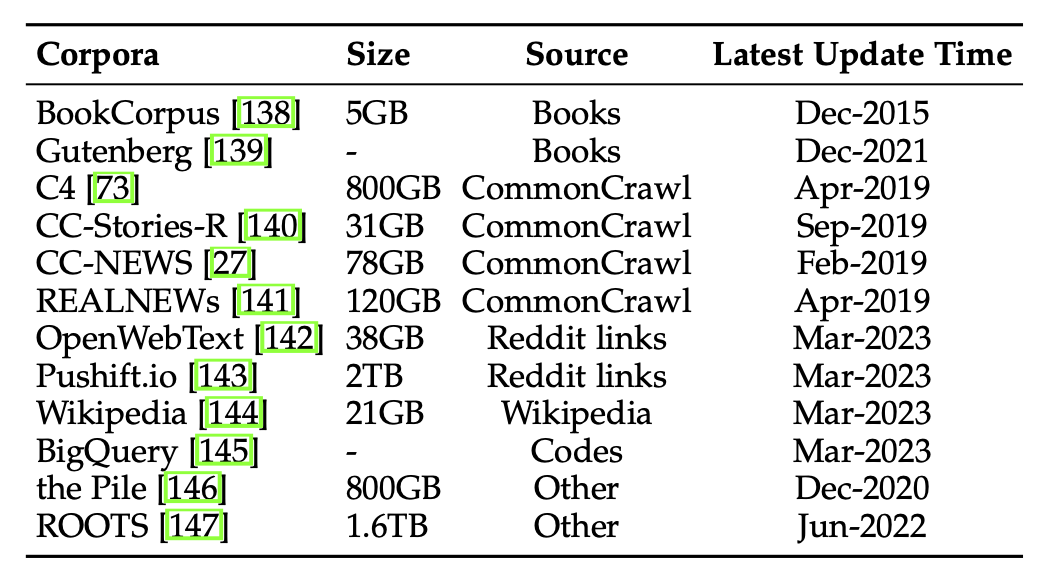
\includegraphics[width=0.99\textwidth]{fig/zhou_2023_tab2}
\caption{Common datasets (Zhou et al., 2023, Table 2)}
\end{figure}

% 1. Data Collection
% use Table 2 Zhao p 11 and part 4.1
% Use Figure 5 here
% Quality filtering: p 14

\end{frame}

\begin{frame}{(Pre-training) Data}

\begin{figure}[h]
\centering
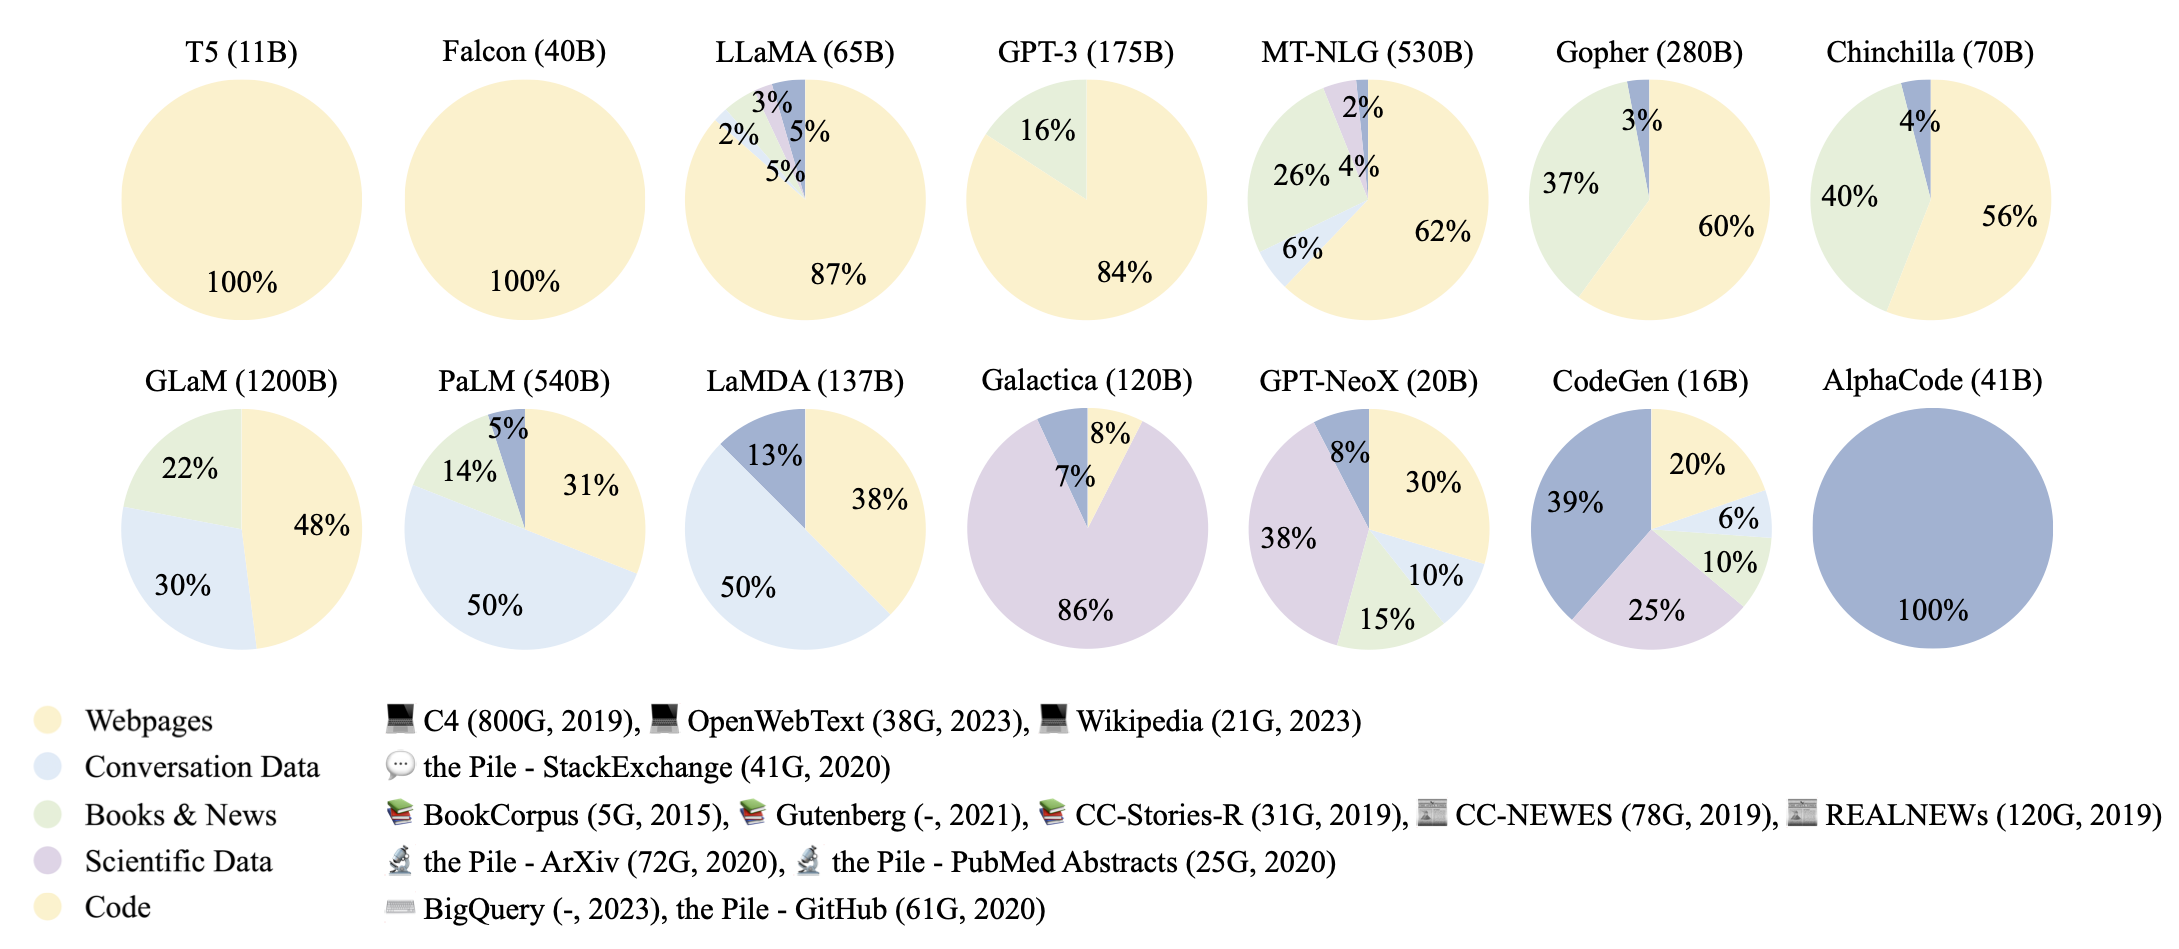
\includegraphics[width=0.99\textwidth]{fig/zhou_2023_fig5}
\caption{Common datasets (Zhou et al., 2023, Figure 5)}
\end{figure}

% 1. Data Collection
% use Table 2 Zhao p 11 and part 4.1
% Use Figure 5 here
% Quality filtering: p 14

\end{frame}

\begin{frame}{(Pre-training) Data}

\begin{figure}[h]
\centering
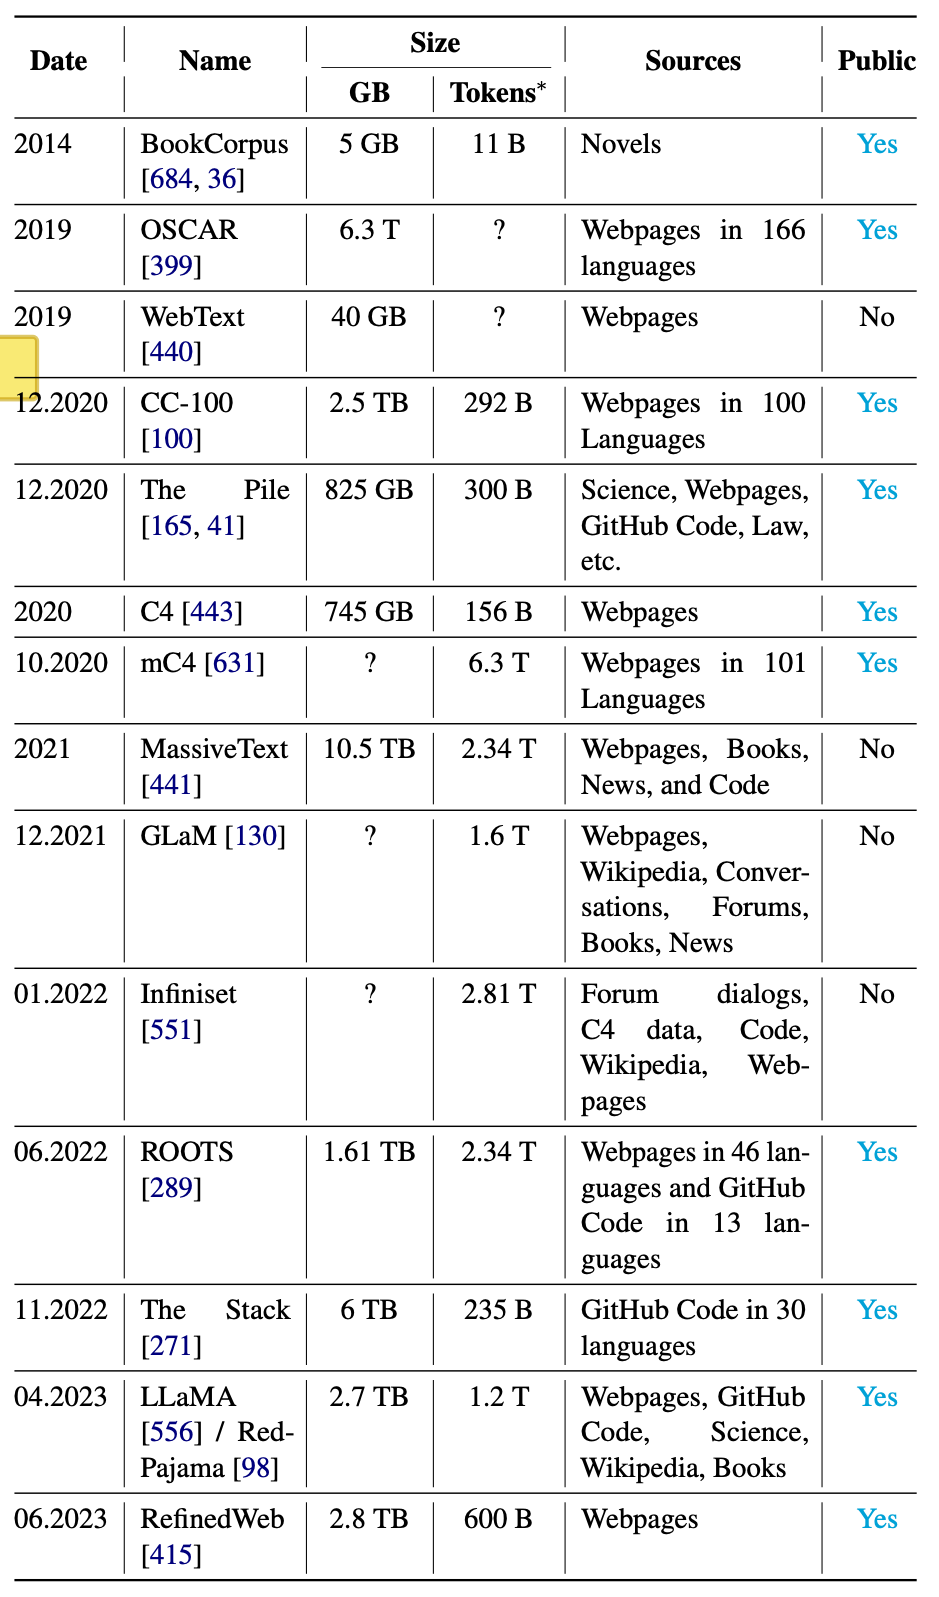
\includegraphics[width=0.45\textwidth]{fig/kaddour_2023_tab1}
\caption{Common datasets (Kaddour et al., 2023, Table 1)}
\end{figure}

\end{frame}


\begin{frame}{(Pre-training) Data}

\begin{figure}[h]
\centering
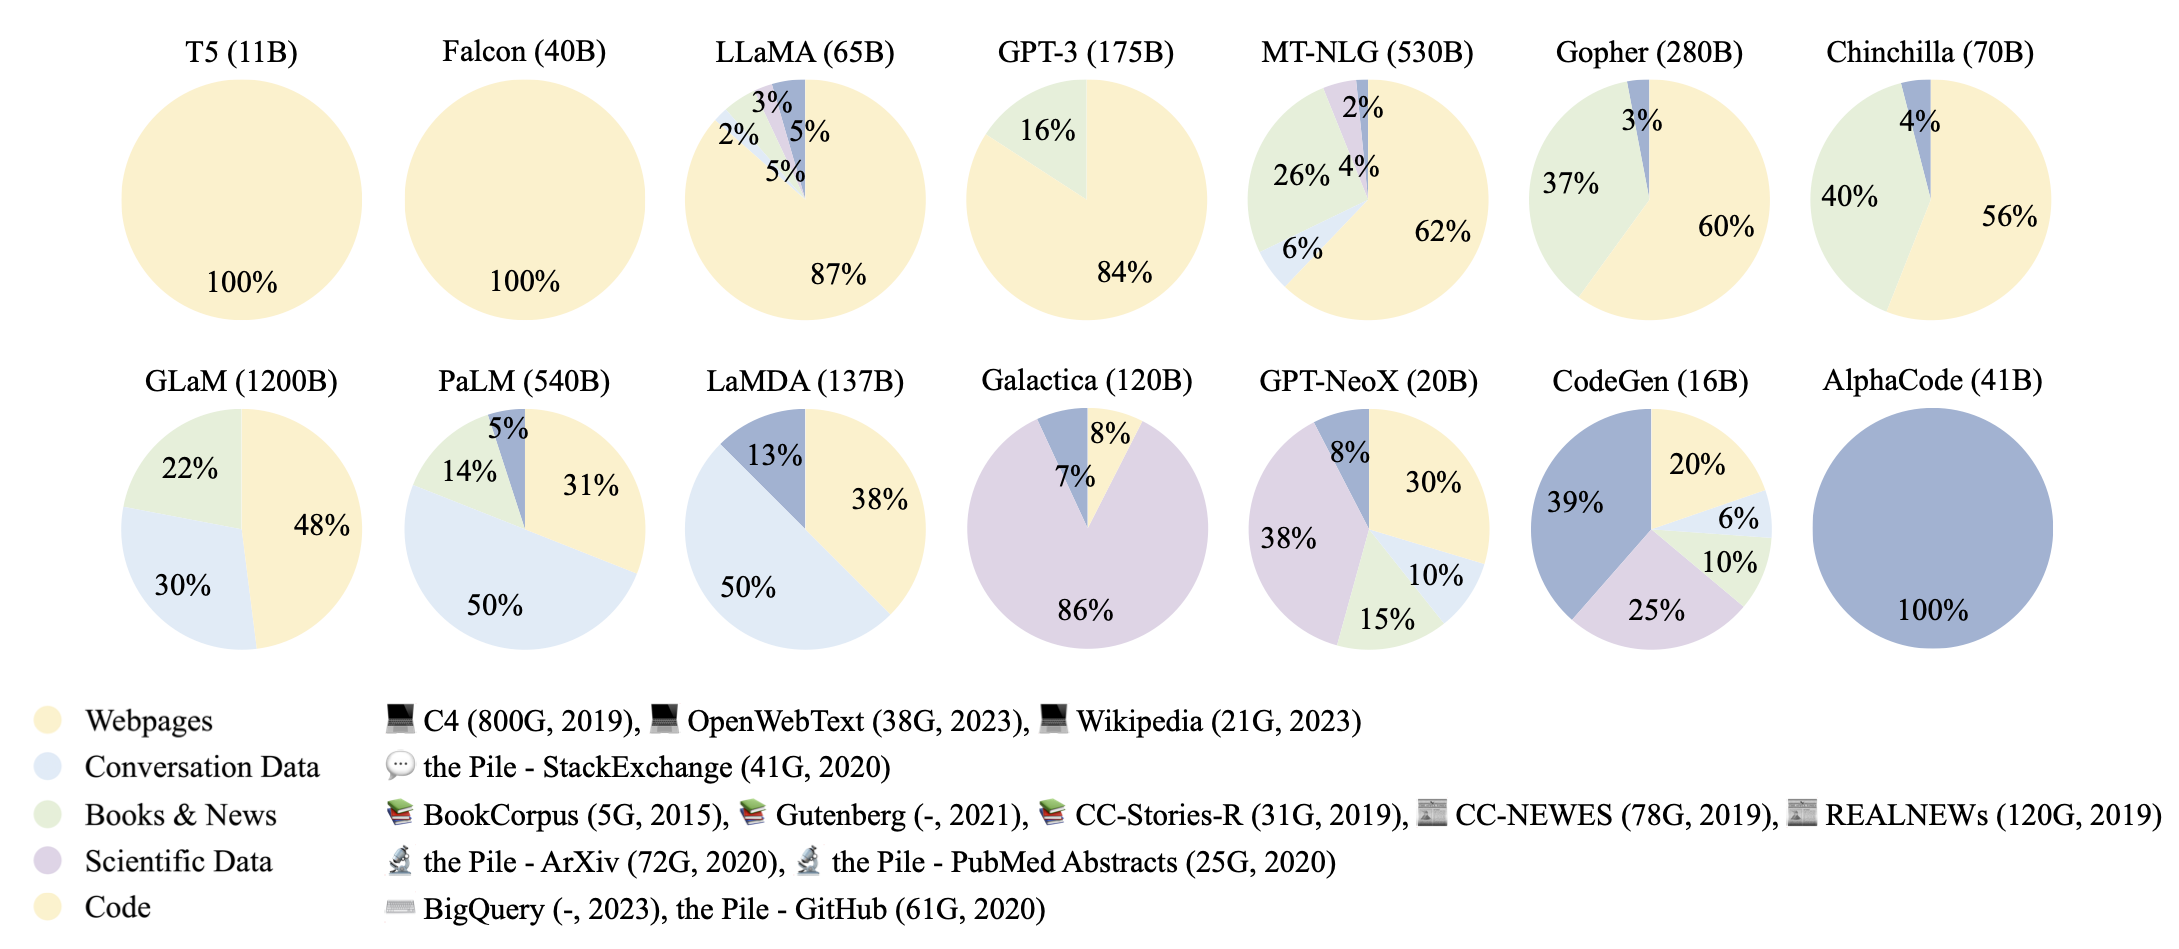
\includegraphics[width=0.99\textwidth]{fig/zhou_2023_fig5}
\caption{Common pretraining datasets (Zhou et al., 2023, Figure 5)}
\end{figure}

\end{frame}


\begin{frame}{Pre-training Data Processing Pipeline}

\begin{figure}[h]
\centering
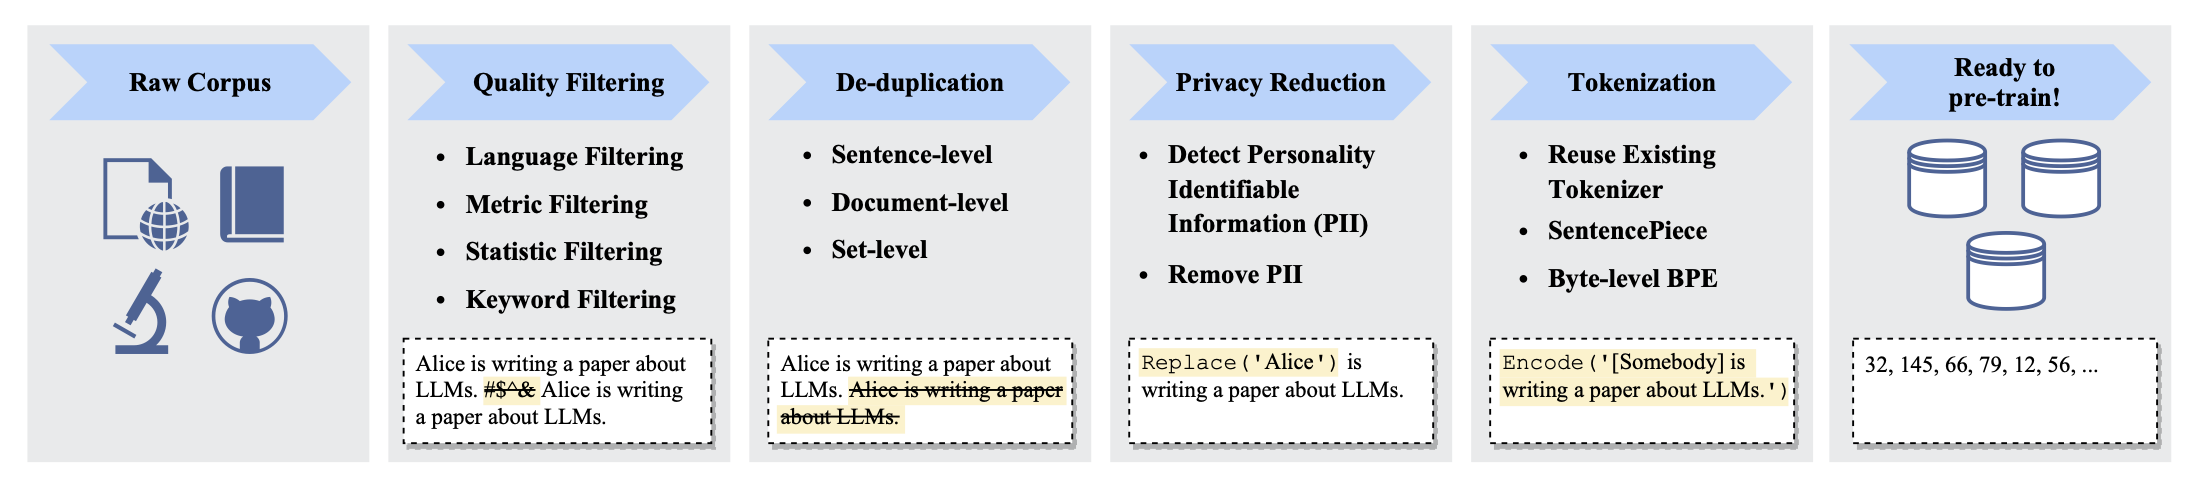
\includegraphics[width=0.99\textwidth]{fig/zhou_2023_fig6}
\caption{Pre-training data processing (Zhou et al., 2023, Figure 6)}
\end{figure}

\end{frame}



\begin{frame}{Tokenization}
% See p. 15
\begin{itemize}
\item Simple tokenization: Word based
\begin{itemize}
\item Difficult in some languages (e.g. Chinese)
\item Generate large vocabularies with many different words
\item Out-of-vocabulary problem
\end{itemize}
\item Byte-pair encoding (BPE): Combine most common characters until predefined vocabulary is reached
\item Wordpiece encoding: Simplary to BPE, but uses a language model to score which to merge
\item Unigram tokenizer: Like wordpiece, but start with a large vocabulary and trim it down.
\end{itemize}

\end{frame}

\begin{frame}{Pretraining task/Loss}

\begin{itemize}
\item The most common task is language modeling(LM), i.e. maximizing
\[
L_{LM}(\mathbf{x}) = \sum_i^n \log P(x_i | \mathbf{x}_{<i})
\]
\item Why is this good?
\begin{itemize}
\item To better and better predict text we need to increase the \uured{understanding} of the model.
\item E.g. "Biden and Xi and a meeting on the role of ..." (artificial intelligence)
\end{itemize}
\end{itemize}


\end{frame}

\begin{frame}{Optimization}

\begin{figure}[h]
\centering
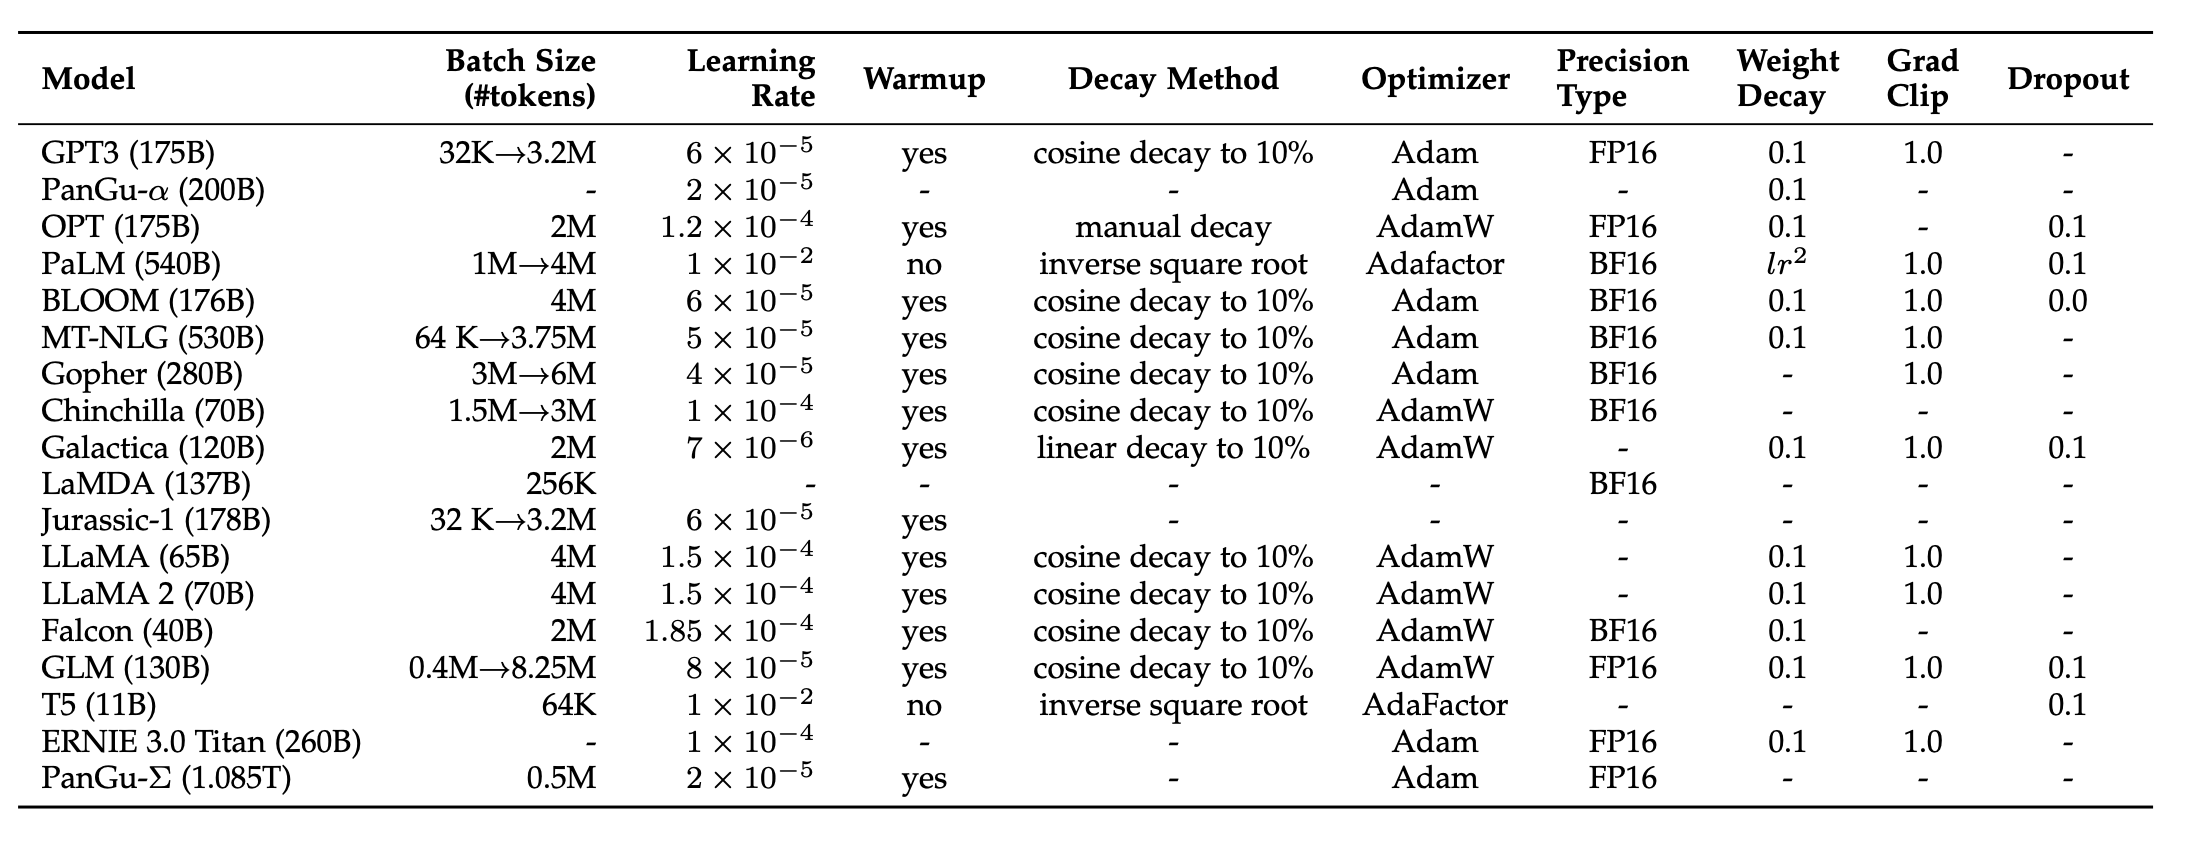
\includegraphics[width=0.99\textwidth]{fig/zhou_2023_tab5}
\caption{Optimization during pre-training (Zhao et al, 2023, Table 5)}
\end{figure}

\end{frame}



\section{Adaptation and Alignment}

\begin{frame}{Instruction tuning/following}

% instruction tuning (discussed in Section 5.1)
\begin{itemize}
\item We have a very large, pre-trained model
\item We want it \uured{perform tasks} (e.g. chatbot): instruction tuning
\item We want it \uured{to be safe}: alignment
\end{itemize}

\end{frame}


\subsection{Instruction tuning}

\begin{frame}{Instruction tuning/following}

% instruction tuning (discussed in Section 5.1)
\begin{itemize}
\item instruction tuning is the approach to fine-tuning pre-trained LLMs on a collection of formatted instances
\item Generally, an instruction-formatted instance consists of a task description (called an instruction), an optional input, the corresponding output, and a small number of demon- strations (optional).
\item For instruction tuning, there are two kinds of important instruction data, namely task-formatted instructions and daily chat instructions.
\item There are multiple ways to create (supervised) data, manual (NLP datasets), using API interactions, creating synthetic data
\item In- struction tuning is an effective approach to adapting existing general LLMs to be domain-specific experts. For instance, researchers propose to fine-tune Flan-PaLM [64] using medi- cal datasets to create Med-PaLM [282], a medical knowledge assistant that achieves performance levels comparable to those of expert clinicians.
\item Key crucial aspects:
\begin{itemize}
\item Scaling - a large number of instances, but the effect is descreasing
\item Including things to avoid, reasons, and suggestions, into instructions may have a negligible or even adverse effect on the performance of LLMs
\item To summarize: diversity and quality of instructions seem to be more important than the number of instances
\end{itemize}
\item Effect: Performance improvement, a general approach to enhancing the abilities of existing language models
\end{itemize}

\end{frame}

\begin{frame}{Instruction tuning training}

% instruction tuning (discussed in Section 5.1)
\begin{itemize}
\item Unlike pre-training, instruction tuning is often more efficient since only a moderate number of instances are used for training.
\item the training objective (i.e., usually sequence-to-sequence loss)
\item e.g., smaller batch size and learning rate)
\item it is important to balance the proportion of different tasks during fine- tuning. A widely used method is the examples-proportional mixing strategy
\item pre-training data during instruction tuning, which can be regarded as regularization for model tuning
\end{itemize}

\end{frame}

\begin{frame}{Fine-tuning Llama}

\begin{figure}[h]
\centering
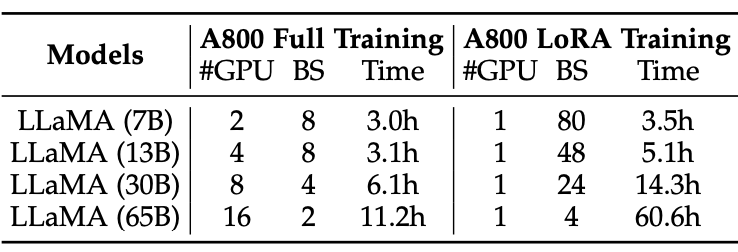
\includegraphics[width=0.99\textwidth]{fig/zhao_2023_tab7}
\caption{Training time for fine-tuning Llama}
\end{figure}

\end{frame}


\subsection{Alignment}

\begin{frame}{Alignment tuning}

% Aligning p 4 in Zhao

\begin{itemize}
\item Problems in LLMs: fabricating false information, producing harmful, misleading, and biased expressions
% LLM may sometimes exhibit unintended behaviors, e.g., fabricating false information, pursuing inaccurate objectives, and producing harmful, misleading, and biased expressions [61, 293].
\item Similar to instruction training, but require different criterias
% However, unlike the original pre-training and adaptation tuning (e.g., instruction tuning), such an alignment requires considering very different crite- ria (e.g., helpfulness, honesty, and harmlessness).
\item The three Hs: helpfulness, honesty, and harmlessness
\item Alignment might harm the general abilities of LLMs to some extent: \uured{alignment tax}%, which is called alignment tax in related literature [295].
\item \uured{Red teaming}: Probe LLMs in an adversarial way to generate harmful outputs and then updates LLMs to prevent such outputs.

\end{itemize}

\end{frame}


\begin{frame}{Alignment tuning: Criterias}

% Aligning p 4 in Zhao
% RLHF

\begin{itemize}
\item Helpfulness
\begin{itemize}
\item To be helpful, the LLM should demon- strate a clear attempt to assist users in solving their tasks or answering questions in a concise and efficient manner as possible.
\end{itemize}
\item Honesty
\begin{itemize}
\item A LLM aligned to be honest should present accurate content to users instead of fabricating information. Additionally, it is crucial for the LLM to convey appropriate degrees of uncertainty in its output, in order to avoid any form of deception or misrepresentation of information. This requires the model to know about its capabilities and levels of knowledge (e.g., “know unknowns”).
\end{itemize}
\item Harmlessness
\begin{itemize}
\item To be harmless, it requires that the language produced by the model should not be offensive or discriminatory. To the best of its abilities, the model should be capable of detecting covert endeavors aimed at soliciting requests for malicious purposes.
\end{itemize}
\end{itemize}

\end{frame}


\begin{frame}{Alignment tuning: Human feedback}

\begin{itemize}
\item High-quality human feedback is extremely important for aligning LLMs with human pref- erences and values.
\item Human Labeler Selection. In existing work, the dominant method for generating human feedback data is human annotation. usually native speakers.
\item Three ways to collect feedback from humans:
\begin{enumerate}
\item Ranking based (choosing the best out of many suggestions)
\item Answering question about the model output (multiple choice)
\item Collect data about if the model is "breaking the rules" helpful, correct, and harmless. (as scores)
\end{enumerate}
\end{itemize}

\end{frame}

\subsection{RLHF}

\begin{frame}{Reinforcement learning with human feedback (RLHF)}
% (discussed in Section 5.2.3)
%The RLHF system mainly comprises three key components: a pre-trained LM to be aligned, a reward model learning from human feedback, and a RL algorithm training the LM.

\begin{itemize}
\item One way to align a model (e.g. in chatGPT)
\item Three components: Human feedback, Reward model training, Fine-tune with reward model.
\item \uured{Idea:} The reward model (RM) learn human preferences
\item  RM: A fine-tuned LM or a LM trained from scratch using human preference data.
\item The reinforcement learning:
\begin{itemize}
\item the (LLM) agent  will perform an action by generate text
\item the (RM) will give the agent a reward signal
\end{itemize}
\end{itemize}

\end{frame}


\begin{frame}{RLHF: Three steps}

\begin{enumerate}
\item Supervised finetuning %To make the LM initially perform desired behaviors, it usually needs to collect a supervised dataset containing input prompts (instruction) and desired outputs for fine-tuning the LM.
\item Learn reward model % : OpenAI uses 6B GPT-3 and DeepMind uses 7B Gopher, but bigger is usually better
\item Fine-tune the model with the reward model
\end{enumerate}

\begin{figure}[h]
\centering
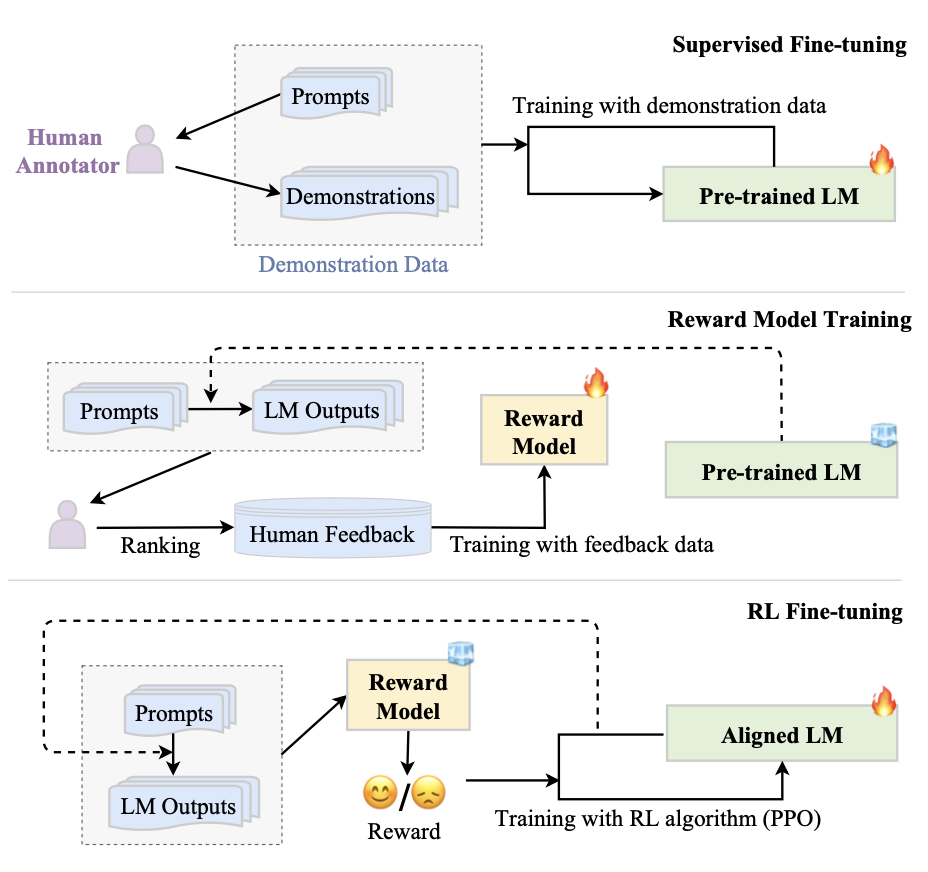
\includegraphics[width=0.99\textwidth]{fig/zhao_2023_fig10}
\caption{RLHF (Zhao, 2023, Figure 10)}
\end{figure}

\end{frame}



\begin{frame}{The values of LLMs}

\begin{itemize}
\item What are the values of an LLM?
\item Atari et al (2023) asked ChatGPT World Value Survey questions:
\end{itemize}
\pause
\begin{figure}[h]
\centering
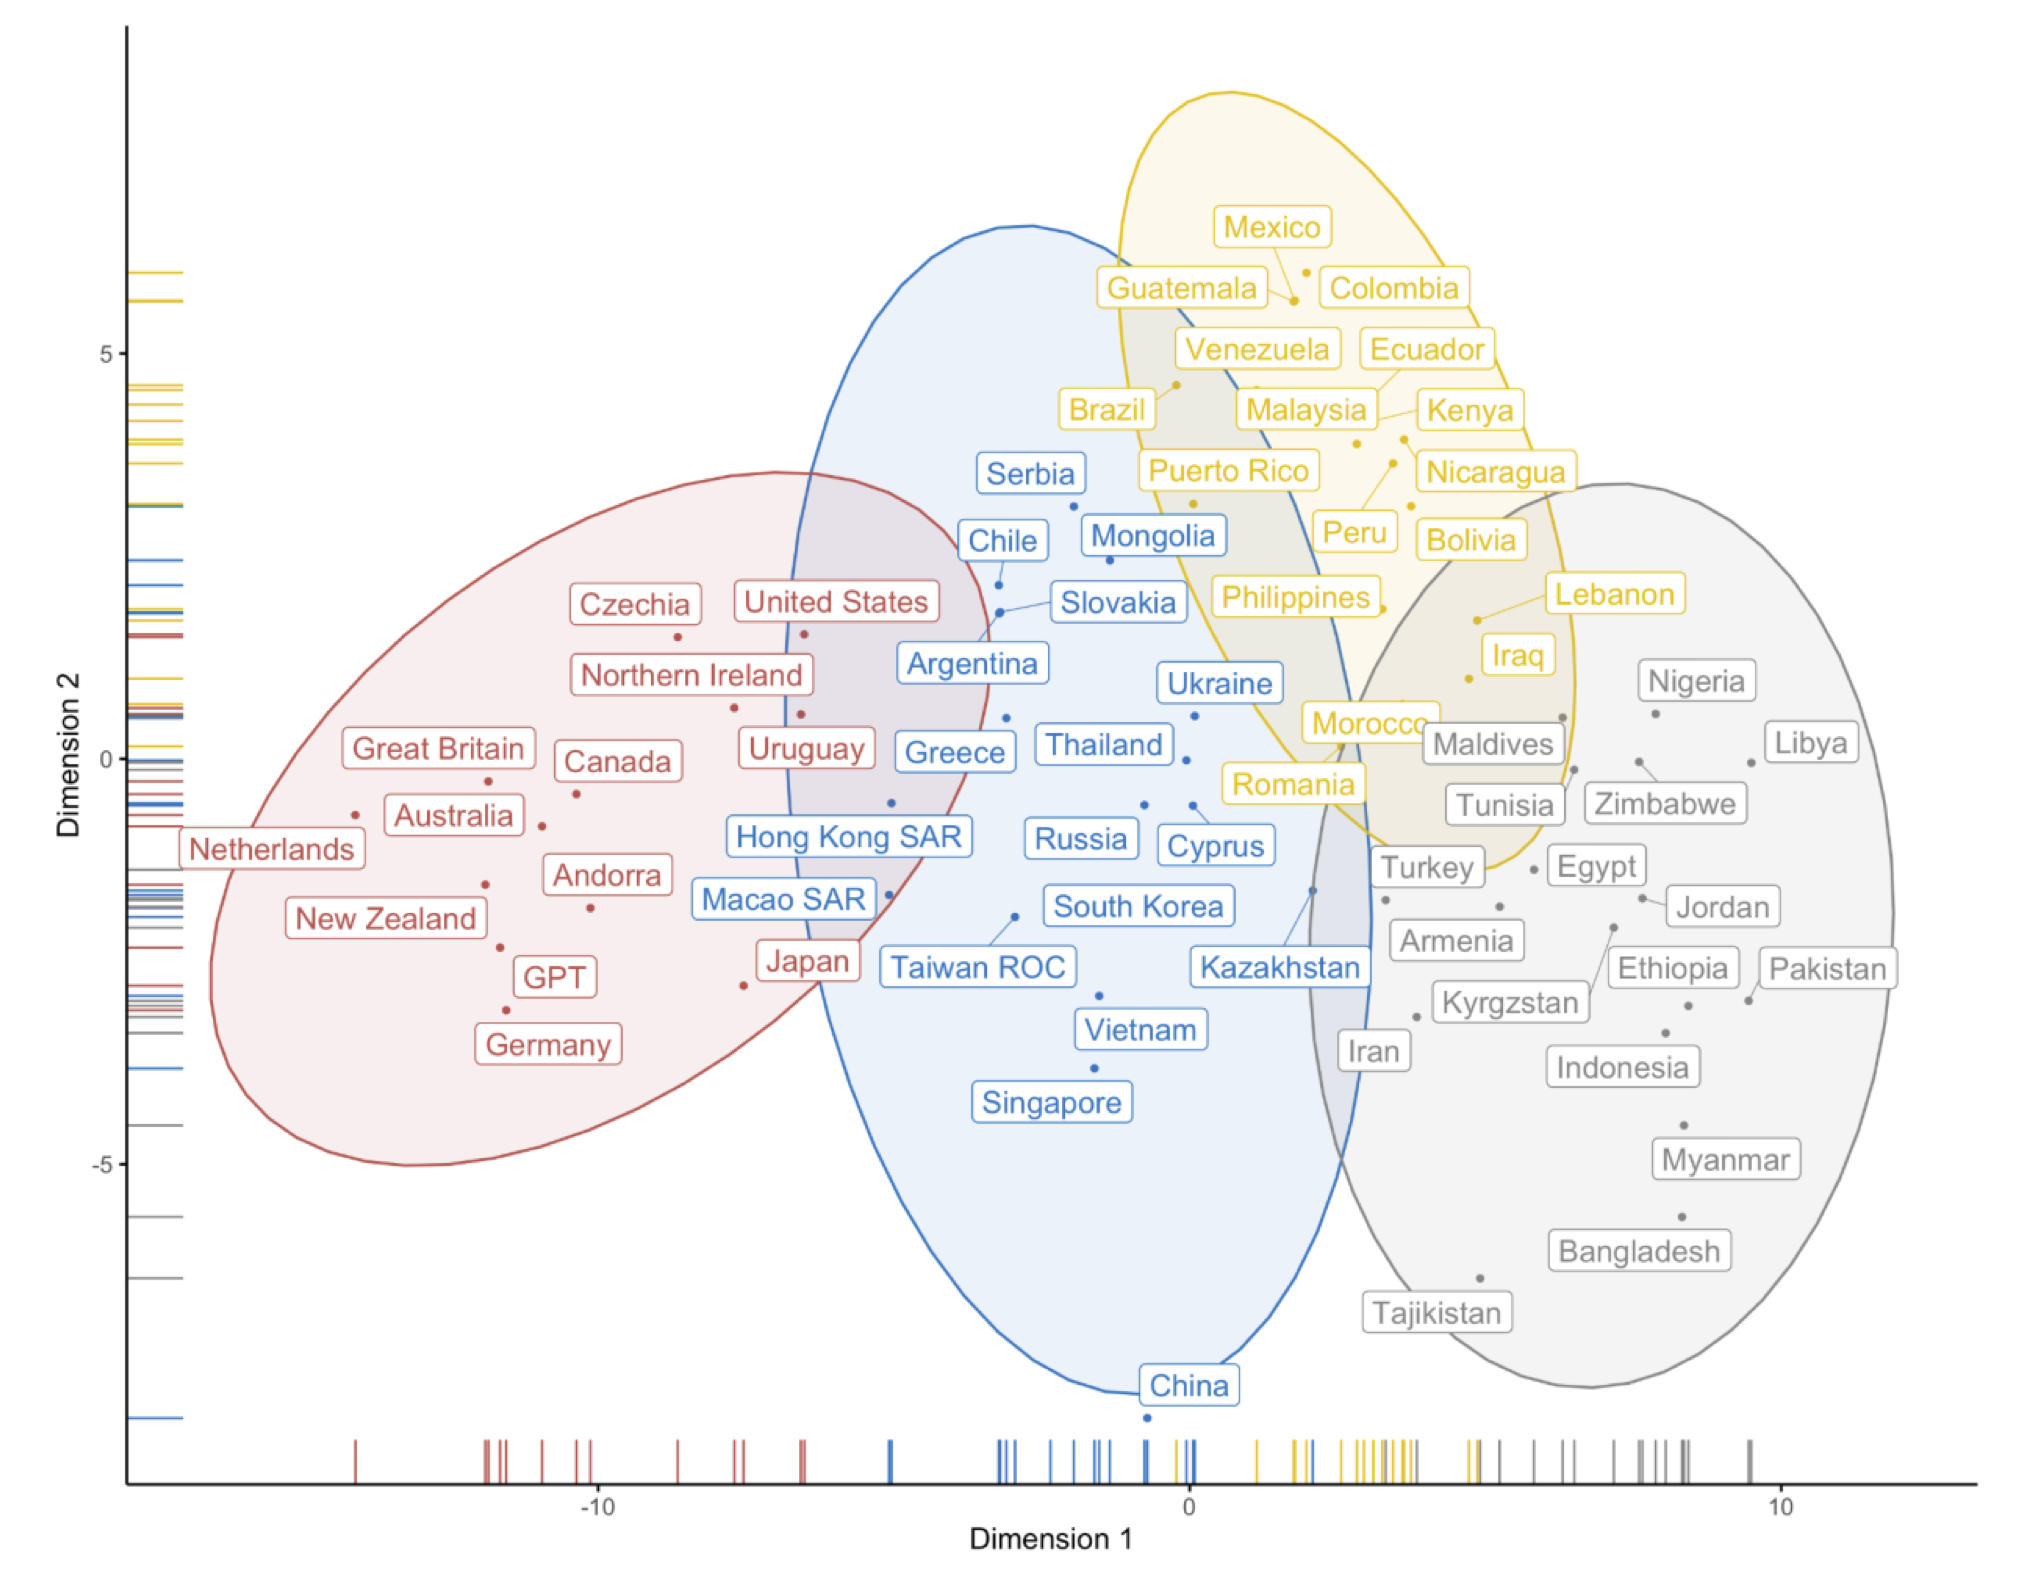
\includegraphics[width=0.8\textwidth]{fig/atari_2023_fig2}
\caption{Value dimensions (Atari et al., 2023, Figure 2)}
\end{figure}


\end{frame}


\section{Usage}

\begin{frame}{Text Generation}
% Kaddour (2023): 3.3

\end{frame}

\begin{frame}{Code Generation}
% Kaddour (2023): 3.3


\end{frame}

\begin{frame}{Text classification}

% The results from Etienne

\end{frame}

% Kaddour (2023): 3.3

\begin{frame}{ChatBots}

% Kaddour (2023): 3.1
%C. Conversational Agents
%1. Chatbots
%2. Virtual Assistants

\end{frame}


\begin{frame}{Law and Generative (AI)}

% Law and AI: 3.6

\end{frame}



\subsection{Prompt engineering}

\begin{frame}{How to prompt}

% take a deep breth and think.
% section 8 Zhao

\end{frame}

\section{Safety and Risks}

\begin{frame}{Risks}

% 1177 chatbot
% See Zhao

\end{frame}


\end{document}
